\documentclass[a4paper,twoside]{article}
\usepackage{autiwa}

\title{Aide mémoire Java}
\author{Autiwa}

\makeindex
\begin{document}

\tableofcontents

\clearpage

\section{Préambule}
Java est un language orienté objet, il n'est pas possible d'y couper. Dans toute la suite, il sera supposé que vous connaissez déjà le principe de la Programmation Orienté Objet (POO). 

En Java, l'exécution d'un programme va lancer la méthode \textbf{main()} de l'objet associé. Le code ci-dessous est le code minimum d'un programme Java qui défini la classe \textbf{sdz1}. Ce code ne fait rien. 
\begin{lstlisting}[language=java]
public class sdz1 {

  /**
  * @param args
  */

  public static void main(String[] args) {
  // TODO Auto-generated method stub

  }
}
\end{lstlisting}

Le même code, affichant le sempiternel ``Hello World'' : 
\begin{lstlisting}[language=java]
import java.util.Scanner;


public class sdz1 {

  /**
    * @param args
    */
  public static void main(String[] args) {
    // TODO Auto-generated method stub
    
    System.out.println("Hello World!");
  }

}
\end{lstlisting}

Quelques informations de base : 
\begin{itemize}
\item Le programme commence par le lancement de la méthode \textbf{.main()} de la classe du programme principal.%TODO expliquer mieux où commence un programme et ce que veut dire le main
\item Les lignes doivent se terminer par ``\textbf{;}''
\item Il faut déclarer les variables avant de les utiliser (voir \refsec{sec:types_variables})
\item Il faut compiler le programme avant de pouvoir l'utiliser (via une plateforme java, ce n'est pas un binaire mais un bytecode utilisable uniquement par un environnement Java)
\end{itemize}


\section{Les bases}
\subsection{Commentaires}
Il existe deux types de commentaires : 
\begin{itemize}
\item les commentaires unilignes : introduits par les symboles \textbf{//}, ils mettent tout ce qui les suit en commentaires, du moment que le texte se trouve sur la même ligne que les \textbf{//}.
\begin{lstlisting}[language=java]
public static void main(String[] args){
  //Un commentaire
  //un autre
  //Encore un autre
  Ceci n'est pas un commentaire ! ! ! !
}
\end{lstlisting}


\item les commentaires multilignes : ils sont introduits par les symboles \textbf{/*} et se terminent par les symboles \textbf{*/}.
\begin{lstlisting}[language=java]
public static void main(String[] args){
 
  /*
  Un commentaire
  Un autre
  Encore un autre
  */
  Ceci n'est pas un commentaire ! ! 
}
\end{lstlisting}
\end{itemize}

\bigskip

Il existe en fait un troisième type de commentaires : les \gras[javadoc]{javadocs}. Ce sont des commentaires avec une mise en forme particulière (ils commencent par \verb|/**| au lieu de \verb|/*|) qui vont permettre de générer de la documentation de manière automatisée. En voici un exemple :
\begin{lstlisting}[language=java]
  /**
   * Retourne une chaine de caracteres selon le resultat de la comparaison
   * @param v1
   *            objet Ville
   * @return comparaison de deux ville
   */
\end{lstlisting}

Dans \gras{Eclipse}, il vous suffit d'aller dans \textbf{Project} et de cliquer sur \textbf{Generate Javadoc}.


\subsection{Types de variables}\label{sec:types_variables}
En Java, nous avons deux type de variables :
\begin{itemize}
\item des variables de type simple ou "primitif"
\item des variables de type complexe : des \textbf{objets}. Le type \gras[type!String]{String} est un type complexe puisque c'est un objet, mais primitif puisque vous n'avez pas à en définir la classe correspondante pour qu'il existe.
\end{itemize}

\subsubsection{Variables primitives}
Ce qu'on appelle des types simples, ou types primitifs, en Java ce sont tout bonnement des nombres entiers, des nombres réels, des booléens ou encore des caractères. 

Commençons par les variables de type numérique
\begin{itemize}
\item Le type \gras[type!byte]{byte} (1 octet) peut contenir les entiers entre $-128$ et $+127$.
\begin{lstlisting}[language=java]
byte temperature;
temperature = 64;
\end{lstlisting}

\item Le type \gras[type!short]{short} (2 octets) contient les entiers compris entre $-32768$ et $+32767$.
\begin{lstlisting}[language=java]
short vitesseMax;
vitesseMax = 32000;
\end{lstlisting}

\item Le type \gras[type!int]{int} (4 octets) va de $-2*10^9$ à $2*10^9$ (2 et 9 zéros derrière...).
\begin{lstlisting}[language=java]
int temperatureSoleil;
temperatureSoleil = 15600000;
\end{lstlisting}
C'est en kelvins...

\item Le type \gras[type!long]{long}(8 octets) de $-9*10^{18}$ à $9*10^{18}$.
\begin{lstlisting}[language=java]
long anneeLumiere;
anneeLumiere = 9460700000000000;
\end{lstlisting}

\item Le type \gras[type!float]{float} (4 octets) correspond à des nombres avec virgule flottante.
\begin{lstlisting}[language=java]
float pi;
pi = 3.141592653f;
\end{lstlisting}
ou encore
\begin{lstlisting}[language=java]
float nombre;
nombre = 2.0f;
\end{lstlisting}

Vous remarquerez que nous ne mettons pas de virgule mais un point ! Et vous remarquerez aussi que même si le nombre en question est rond, on met tout de même .0 derrière celui-ci !

\item Le type \gras[type!double]{double} (8 octets) est identique à float, si ce n'est qu'il contient un nombre plus grand derrière la virgule.
\begin{lstlisting}[language=java]
double division;
division = 0.333333333333333333333333333333333333333333334;
\end{lstlisting}
\end{itemize}

\bigskip

Le type \gras[type!char]{char} contient UN caractère stocké entre de simples quotes ' ' comme ceci...
\begin{lstlisting}[language=java]
char caractere;
caractere = 'A';
\end{lstlisting}

\bigskip

Le type \gras[type!boolean]{boolean} qui lui contient \textbf{true} (vrai) ou \textbf{false} (faux).
\begin{lstlisting}[language=java]
boolean question;
question = true;
\end{lstlisting}

\subsubsection{Astuces}
On peut très bien compacter la phase de déclaration et d'initialisation en une seule phase ! Comme ceci :
\begin{lstlisting}[language=java]
int entier = 32;
float pi = 3.1416f;
char carac = 'z';
String mot = new String("Coucou");
\end{lstlisting}

Et lorsque nous avons plusieurs variables d'un même type, nous pouvons compacter tout ceci en une déclaration comme suit :
\begin{lstlisting}[language=java]
int nbre1 = 2, nbre2 = 3, nbre3 = 0;
\end{lstlisting}

\bigskip

On peut aussi convertir une variable ou une formule dans un autre type de donnée via ce qu'on appelle un \textbf{cast} :
\begin{lstlisting}[language=java]
int i = 123;
double j = (double)i;
\end{lstlisting}

\begin{attention}
Il peut y avoir des pertes de précision au sein même des opérations mathématiques que la conversion du résultat via un cast n'empêchera pas. 
Ex :
\begin{lstlisting}[language=java]
int i = 123, j = 5;
double k = (double) (i / j);
\end{lstlisting}
\end{attention}

\subsubsection{Un type complexe particulier : la Chaîne de caractères}
Le type \gras[type!String]{String} correspond à de la chaîne de caractères.
Ici, il ne s'agit pas d'une variable mais d'un objet qui instancie une classe qui existe dans Java ; nous pouvons l'initialiser en utilisant l'opérateur unaire \gras{new()} dont on se sert pour réserver un emplacement mémoire à un objet, ou alors lui affecter directement la chaîne de caractères.

Vous verrez que celle-ci s'utilise très facilement et se déclare comme ceci :
\begin{lstlisting}[language=java]
String phrase;
phrase = "Titi et gros minet";
//Deuxieme methode de declaration de type String
String str = new String();
str = "Une autre chaine de caracteres";
//La troisieme
String string = "Une autre chaine";
//Et une quatrieme pour la route
String chaine = new String("Et une de plus ! ");
\end{lstlisting}

\bigskip

\gras[type!String]{String} étant un objet, il possède des méthodes afin de les manipuler. En voici quelques exemples :
\begin{itemize}

\item \gras{toLowerCase()}

Cette méthode permet de transformer toute saisie clavier de type caractère en minuscules. Elle n'a aucun effet sur les nombres, puisqu'ils ne sont pas assujettis à cette contrainte. Vous pouvez donc utiliser cette fonction sur une chaîne de caractères comportant des nombres.
Elle s'utilise comme ceci :
\begin{lstlisting}[language=java]
String chaine = new String("COUCOU TOUT LE MONDE !");
String chaine2 = new String();
chaine2 = chaine.toLowerCase();//donne "coucou tout le monde !"
\end{lstlisting}


\item \gras{toUpperCase()}

Il s'agit de l'opposée de la précédente. Elle transforme donc une chaîne de caractères en majuscules. Et s'utilise comme suit :
\begin{lstlisting}[language=java]
String chaine = new String("coucou coucou"), chaine2 = new String();
chaine2 = chaine.toUpperCase();//donne "COUCOU COUCOU"
\end{lstlisting}


\item \gras{concat()}

Cette méthode permet de concaténer deux chaînes de caractères.
\begin{lstlisting}[language=java]
String str1 = new String("Coucou "), str2 = new String("toi !");
String str3 = new String();
str3 = str1.concat(str2);//donne "Coucou toi !"
\end{lstlisting}


\item \gras{length()}

Celle-là permet de donner la longueur d'une chaîne de caractères (en comptant les espaces blancs).
\begin{lstlisting}[language=java]
String chaine = new String("coucou ! "); 
int longueur = 0;
longueur = chaine.length();//donne 9
\end{lstlisting}


\item \gras{equals()}

Permet de voir si deux chaînes de caractères sont identiques. Donc, de faire des tests. C'est avec cette fonction que vous ferez vos tests de conditions, lorsqu'il y aura des \gras[type!String]{String}. Exemple concret :
\begin{lstlisting}[language=java]
String str1 = new String("coucou"), str2 = new String("toutou");
 
if (str1.equals(str2))//Si les deux chaines sont identiques
        System.out.println("Les deux chaines sont identiques !");
 
else
        System.out.println("Les deux chaines sont differentes !");
\end{lstlisting}


Vous pouvez aussi demander la non vérification de l'égalité grâce à l'opérateur de négation \og !\fg, ce qui nous donne :
\begin{lstlisting}[language=java]
String str1 = new String("coucou"), str2 = new String("toutou");
 
if (!str1.equals(str2))//Si les deux chaines sont differentes
        System.out.println("Les deux chaines sont differentes !");
 
else
        System.out.println("Les deux chaines sont identiques !");
\end{lstlisting}

Le principe de ce genre de condition fonctionne de la même façon pour les boucles. Et dans l'absolu, cette fonction retourne un booléen. C'est pourquoi nous pouvons utiliser cette fonction dans les tests de condition.
\begin{lstlisting}[language=java]
String str1 = new String("coucou"), str2 = new String("toutou");
boolean Bok = str1.equals(str2);//ici Bok prendra la valeur false
\end{lstlisting}

\item \gras{charAt()}

Le résultat de cette méthode sera un caractère, car il s'agit d'une méthode d'extraction de caractères, je dirais même d'UN caractère. Elle ne peut s'opérer que sur des \gras[type!String]{String}! Elle possède la même particularité que les tableaux, c'est-à-dire que, pour cette méthode, le premier caractère sera le numéro 0. Cette méthode prend un entier comme argument.
\begin{lstlisting}[language=java]
String nbre = new String("1234567");
char carac = ' ';
carac = nbre.charAt(4);//renverra ici le caractere 5
\end{lstlisting}


\item \gras{substring()}

Comme son nom l'indique, elle permet d'extraire une sous-chaîne de caractères d'une chaîne de caractères. Cette méthode prend 2 entiers comme arguments. Le premier définit le début de la sous-chaîne à extraire inclus, le deuxième correspond au dernier caractère à extraire exclus. Et le premier caractère est aussi le numéro 0.
\begin{lstlisting}[language=java]
String chaine = new String("la paix niche"), chaine2 = new String();
chaine2 = chaine.substring(3,13);//permet d'extraire "paix niche"
\end{lstlisting}


\item \gras{indexOf()}/\gras{lastIndexOf()}

\gras{indexOf()} permet d'explorer une chaîne de caractères depuis son début. \gras{lastIndexOf()} depuis sa fin, mais renvoie l'index depuis le début de la chaine. Elle prend un caractère, ou une chaîne de caractères comme argument, et renvoie un int. Tout comme \gras{charAt()} et \gras{substring()}, le premier caractère est à la place 0. Je crois qu'ici un exemple s'impose, plus encore que pour les autres fonctions :
\begin{lstlisting}[language=java]
String mot = new String("anticonstitutionnellement");
int n = 0;
 
n = mot.indexOf('t');      // n vaut 2
n = mot.lastIndexOf('t');        // n vaut 24
n = mot.indexOf("ti");    // n vaut 2
n = mot.lastIndexOf("ti");      // n vaut 12
n = mot.indexOf('x');      // n vaut -1
\end{lstlisting}
\end{itemize}

\subsubsection{Les types complexes}
Les types complexes, ou objets se déclarent un peu différemment des types primitifs. En effet, la déclaration est en fait une instanciation, c'est à dire qu'on crée un objet appartenant à une certaine classe d'objet :
\begin{lstlisting}[language=java]
Ville bdx = new Ville();
\end{lstlisting}
On définit ici la variable \textbf{bdx} comme étant un objet de la classe \textbf{Ville} à laquelle on affecte l'instanciation \textbf{new Ville()}. \gras{new} signifie qu'on créer un nouvel objet de la classe, le constructeur étant appelé sans aucun argument (vu que les parenthèses n'en contiennent pas). Pour plus de détails sur ce point, voir \refsec{sec:les_classes}.

\subsection{Entrées clavier}
Afin de récupérer ce qu'on tape au clavier, il faut importer une nouvelle classe
\begin{lstlisting}[language=java]
import java.util.Scanner;
\end{lstlisting}

\bigskip

Voici l'instruction pour permettre à Java de récupérer ce que vous avez saisi et ensuite de l'afficher :
\begin{lstlisting}[language=java]
Scanner sc = new Scanner(System.in);
System.out.println("Veuillez saisir un mot :");
String str = sc.nextLine();
System.out.println("Vous avez saisi : " + str);
\end{lstlisting}

\bigskip

Dans le cas où on récupère autre chose qu'une chaîne de caractère, il faut vider la ligne via un \texttt{sc.nextLine();} avant de chercher à récupérer une chaîne de caractère.
\begin{lstlisting}[language=java]
Scanner sc = new Scanner(System.in);

System.out.println("Saisissez un entier : ");
int i = sc.nextInt();

System.out.println("Saisissez une chaine : ");
//On vide la ligne avant d'en lire une autre
sc.nextLine();
String str = sc.nextLine();
System.out.println("FIN ! ");
\end{lstlisting}

\subsection{Opérateur ternaire}\index{opérateur ternaire}
La particularité des conditions ternaires réside dans le fait que trois opérandes (variable ou constante) sont mises en jeu mais aussi que ces conditions sont employées pour affecter des données dans une variable. Voici à quoi ressemble la structure de ce type de condition :
\begin{lstlisting}[language=java]
int x = 10, y = 20;
int max = (x < y) ? y : x ; //Maintenant max vaut 20
\end{lstlisting}

On peut faire par exemple : 
\begin{lstlisting}[language=java]
int x = 10;
String type = (x % 2 == 0) ? "C' est pair" : "C' est impair" ; 
//Ici type vaut "C' est pair"

x = 9;
type = (x % 2 == 0) ? "C' est pair" : "C' est impair" ; 
//Ici type vaut "C' est impair"
\end{lstlisting}

\subsection{Boucles}
\subsubsection{Boucle if}\index{boucle!if}
\begin{lstlisting}[language=java]
if(//condition)
  {
  // execution des instructions si la condition est remplie
  
  
  }
else
  {
  // execution des instructions si la condition n'est pas remplie
  
  
  }
\end{lstlisting}

\begin{exemple}
\begin{lstlisting}[language=java]
int i = 10;
 
if (i < 0)
  System.out.println("Le nombre est negatif");
 
else
  System.out.println("Le nombre est positif");
\end{lstlisting}
\end{exemple}

\begin{remarque}
On n'est pas obligés de mettre les accolades quand il n'y a qu'une seule ligne d'instruction dans la boucle.
\end{remarque}

\bigskip

On peut aussi mettre des tests multiples :
\begin{lstlisting}[language=java]
int i = 0;

if (i < 0)
  System.out.println("Ce nombre est negatif !");      

else if(i > 0)
  System.out.println("Ce nombre est positif !!");           

else  
  System.out.println("Ce nombre est nul !!");
\end{lstlisting}

Si on souhaite faire beaucoup de tests, on peut souhaiter utiliser la structure \gras[boucle!switch]{switch} à la place.

\subsubsection{Boucle Switch}\index{boucle!switch}

\begin{lstlisting}[language=java]
int nbre = 5; 

switch (nbre)
{
  case 1: 
    System.out.println("Ce nombre est tout petit");
    break;

  case 2: 
    System.out.println("Ce nombre est tout petit");
    break;

  case 3: 
    System.out.println("Ce nombre est un peu plus grand");
    break;

  case 4: 
    System.out.println("Ce nombre est un peu plus grand");
    break;

  case 5: 
    System.out.println("Ce nombre est la moyenne");
    break;

  case 6: 
    System.out.println("Ce nombre est tout de meme grand");
    break;

  case 7: 
    System.out.println("Ce nombre est grand");
    break;

  default: 
    System.out.println("Ce nombre est compris entre 8 et 10");

}
\end{lstlisting}

\subsubsection{Boucle while}\index{boucle!while}
\begin{lstlisting}[language=java]
int a = 1, b = 15;
while (a < b)
{
        System.out.println("coucou " +a+ " fois !!");
        a++;
}
\end{lstlisting}

On peut aussi faire :
\begin{lstlisting}[language=java]
//Une variable vide
String prenom;
// On initialise celle-ci a O pour oui !
char reponse = 'O';
//Notre objet Scanner, n'oubliez pas l'import de java.util.Scanner
Scanner sc = new Scanner(System.in);
//Tant que la reponse donnee est egale a oui
while (reponse == 'O')
{
  //On affiche une instruction
  System.out.println("Donnez un prenom : ");
  //On recupere le prenom saisi
  prenom = sc.nextLine();
  // On affiche notre phrase avec le prenom
  System.out.println("Bonjour " +prenom+ " comment vas-tu ?");
  //On demande si la personne veut faire un autre essai
  System.out.println("Voulez-vous reessayer ?(O/N)");
  //On recupere la reponse de l'utilisateur
  reponse = sc.nextLine().charAt(0);
}
 
System.out.println("Au revoir...");
//Fin de la boucle
\end{lstlisting}

\subsubsection{Boucle do while}\index{boucle!do while}
\begin{lstlisting}[language=java]
do{
  blablablablablablablabla
}while(a < b);
\end{lstlisting}

\subsubsection{Boucle for}\index{boucle!for}
\begin{lstlisting}[language=java]
for(int i = 1; i <= 10; i++)
{
  System.out.println("Voici la ligne "+i);
}
\end{lstlisting}

\bigskip

On peut aussi boucler sur les éléments d'un tableau :
\begin{lstlisting}[language=java]
String tab[] = {"toto", "titi", "tutu", "tete", "tata"};
 
for(String str : tab)
   System.out.println(str);
\end{lstlisting}\index{tableaux}

Cette forme de boucle \textbf{for} est particulièrement adaptée au parcours de tableau. On peut naturellement se demander comment faire de même pour des tableaux multidimensionnels. La chose à retenir est que la variable en premier paramètre de la boucle \textbf{for} doit être du même type que la valeur de retour du tableau. Dans le cas d'un tableau multi-dimensionnel, cette dernière sera un tableau de dimension inférieure. En conséquence, on peut boucler sur des sous tableaux, puis sur les éléments de ces derniers via des boucles imbriquées :
\begin{lstlisting}[language=java]
String tab[][] = {{"toto", "titi", "tutu", "tete", "tata"}, 
                  {"1", "2", "3", "4"}};
int i = 0, j = 0;

for(String sousTab[] : tab)
{
  i = 0;
  for(String str : sousTab)
  {     
    System.out.println("La valeur de la nouvelle boucle est : " + str);
    System.out.println("La valeur du tableau a l'indice [" 
      + j + "][" +i +"] est : " +  tab[j][i] + "\n");
    i++;
  }
  j++;
}
\end{lstlisting}

\subsection{Tableaux}\index{tableaux}
On définit des tableaux de la même manière que les éléments qui le constituent. Un tableau a donc un type associé et ne peut stocker que des éléments de ce type là.

Pour définir un tableau sans l'initialiser on fait :
\begin{lstlisting}[language=java]
int tableauEntier[] = new int[6];
//ou encore
int[] tableauEntier2 = new int[6];
\end{lstlisting}
mais la définition d'un tableau initialisé se fait elle de la façon suivante :
\begin{lstlisting}[language=java]
String tableauChaine[] = {"chaine1", "chaine2", "chaine3" , "chaine4"};
\end{lstlisting}

\bigskip

On peut définir des tableaux multi-dimensionnels : 
\begin{lstlisting}[language=java]
int premiersNombres[][] = { {0,2,4,6,8},{1,3,5,7,9} };
\end{lstlisting}

Nous voyons bien ici les deux lignes de notre tableau symbolisées par les doubles crochets \texttt{[][]}. Ce genre de tableau n'est rien d'autre que plusieurs tableaux en un. Ainsi, pour passer d'une ligne à l'autre, nous jouerons avec la valeur du premier crochet.
\begin{exemple}
\verb|premiersNombres[0][0]| correspondra au premier élément de la colonne paire.\\
Et \verb|premiersNombres[1][0]| correspondra au premier élément de la colonne impaire.
\end{exemple}

\begin{remarque}
La longueur d'un tableau \textbf{tab} est donnée par :
\begin{lstlisting}[language=java]
tab.length
\end{lstlisting}
\end{remarque}

\begin{important}
On peut définir des sortes de tableaux pouvant contenir n'importe quel type de données, ce sont des objets de type \gras{ArrayList} qu'on appelle des \gras{collection d'objet}. %TODO parler des ArrayList
\end{important}


\section{Les classes}\label{sec:les_classes}
Toute classe possède un constructeur (une méthode particulière, lancée lors de l'initialisation d'une instance de classe), ayant le même nom que la classe elle-même.

Prenons un exemple avec une classe \textbf{Ville} :
\begin{lstlisting}[language=java]
public class Ville{
  /**
  * Stocke le nom de notre ville
  */
  String nomVille;
  /**
  * Stocke le nom du pays de notre ville
  */
  String nomPays;
  /**
  * Stocke le nombre d'habitants de notre ville
  */
  int nbreHabitant;
 
  /**
   * Constructeur par defaut
   */
  public Ville(){
    System.out.println("Creation d'une ville !");      
    nomVille = "Inconnu";
    nomPays = "Inconnu";
    nbreHabitant = 0;
  }
 
}
\end{lstlisting}

\begin{remarque}
Il est possible de surcharger \refsec{sec:surcharge} le constructeur et ainsi avoir plusieurs constructeurs en fonction des paramètres passés lors de l'initialisation de l'instance de classe.
\end{remarque}

\bigskip

La création d'une instance de classe se fait via le mot clé \textbf{new} :
\begin{lstlisting}[language=java]
Ville bordeaux = new Ville();
\end{lstlisting}

\subsection{Bien gérer les variables}\label{sec:good_behavior}

Dans l'exemple précédent, les \gras[variable!d'instance]{variables d'instance} sont publiques et modifiables directement. La philosophie de la POO est d'utiliser des \gras[accesseur]{accesseurs} getVar (qui renvoient la valeur d'une variable var) et des \gras[mutateur]{mutateurs} setVar (qui modifient la valeur de la variable var). En conséquence, on mettra plutôt les variables avec une portée privée, et on créera des méthodes permettant d'afficher ou modifier ces dernières. La classe devient alors :
\raggedbottom
\begin{lstlisting}[language=java]
public class Ville {
  /**
  * Stocke le nom de notre ville
  */
  private String nomVille;
  /**
  * Stocke le nom du pays de notre ville
  */
  private String nomPays;
  /**
  * Stocke le nombre d'habitants de notre ville
  */
  private int nbreHabitant;

  /**
  * Constructeur par defaut
  */
  public Ville(){
    System.out.println("Creation d'une ville !");          
    nomVille = "Inconnu";
    nomPays = "Inconnu";
    nbreHabitant = 0;
  }
 
  /**
  * Constructeur d'initialisation
  * @param pNom 
  *                    Nom de la Ville
  *  @param pNbre
  *                    Nombre d'habitants
  *  @param pPays
  *                    Nom du pays
  */
  public Ville(String pNom, int pNbre, String pPays)
  {
    System.out.println("Creation d'une ville avec des parametres !");     
    nomVille = pNom;
    nomPays = pPays;
    nbreHabitant = pNbre;
  }
  
 //************************************************************************
  //                                    ACCESSEURS
  //***********************************************************************
  
  /**
   * Retourne le nom de la ville
   * @return le nom de la ville
   */
  public String getNom()
  {
    return nomVille;
  }
  
  /**
   * Retourne le nom du pays
   * @return le nom du pays
   */
  public String getNomPays()
  {
    return nomPays;
  }
  
  /**
   * Retourne le nombre d'habitants
   * @return nombre d'habitants
   */
 public int getNombreHabitant()
 {
    return nbreHabitant;
 }
 
 //************************************************************************
 //                                    MUTATEURS
 //************************************************************************
 
 /**
  * Definit le nom de la ville
  * @param pNom
  *             nom de la ville
  */
 public void setNom(String pNom)
 {
    nomVille = pNom;
 }
 
 /**
  * Definit le nom du pays
  * @param pPays
  *             nom du pays
  */
 public void setNomPays(String pPays)
 {
    nomPays = pPays;
 }
 
 /**
  * Definit le nombre d'habitants
  * @param nbre
  *             nombre d'habitants
  */
  public void setNombreHabitant(int nbre)
  {
    nbreHabitant = nbre;
  }
  
}
\end{lstlisting}
\flushbottom

\subsection{Portée des variables}
Lors de la déclaration de variables ou de méthodes, il y a plusieurs attributs possible, dont le type bien entendu (mais que je ne détaillerai pas ici). 

\bigskip

L'un des attributs est la \textbf{portée} de la variable ou la méthode :
\begin{itemize}
\item \gras{public} : La variable/méthode est accessible par tout le monde
\item \gras{private} : La variable/méthode n'est accessible qu'à l'intérieur de la classe où elle est définie
\item \gras{protected} : La variable/méthode est accessible à l'intérieur de la classe où elle est définie ainsi que toutes ses classes dérivées (\gras{héritage})
\end{itemize}

\begin{figure}[htb]
\centering
\subfloat[Variable publique : accès pour tout le monde]{\label{fig:portee_public}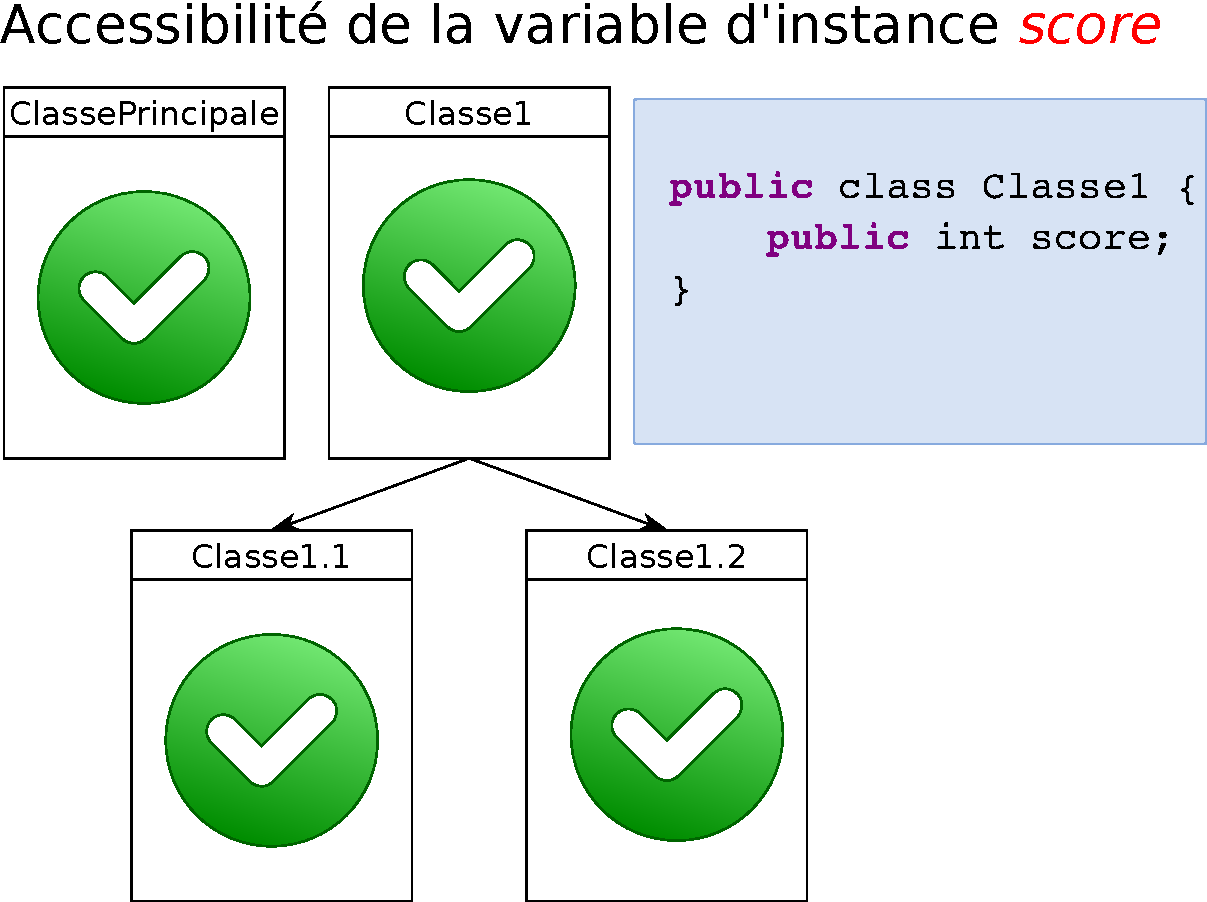
\includegraphics[width=0.3\textwidth]{figures/portee_public.pdf}}\hfill
\subfloat[Variable protégée : accès réservé à la classe et ses classes dérivées]{\label{fig:portee_protected}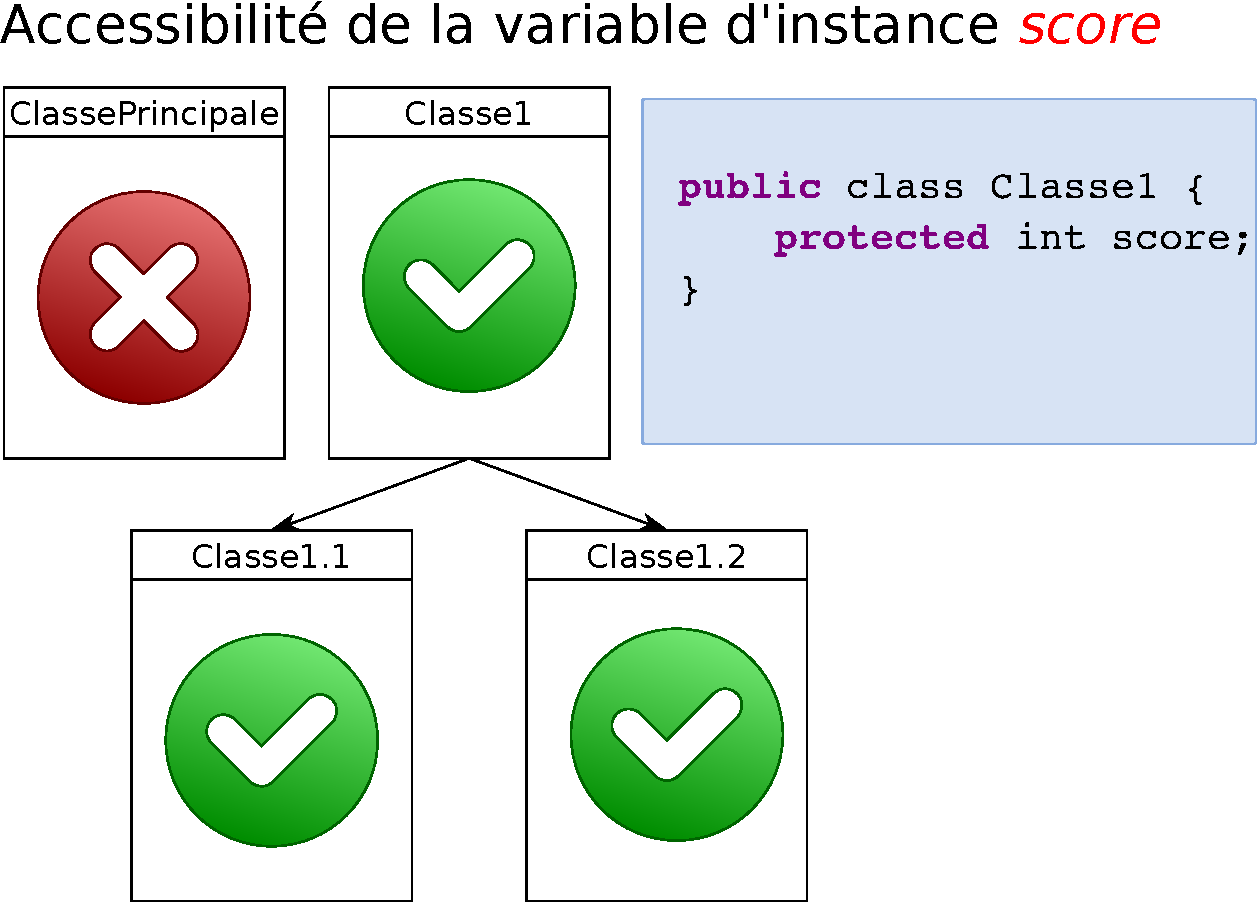
\includegraphics[width=0.3\textwidth]{figures/portee_protected.pdf}}\hfill
\subfloat[Variable privée : accessible uniquement à l'intérieur de la classe.]{\label{fig:portee_private}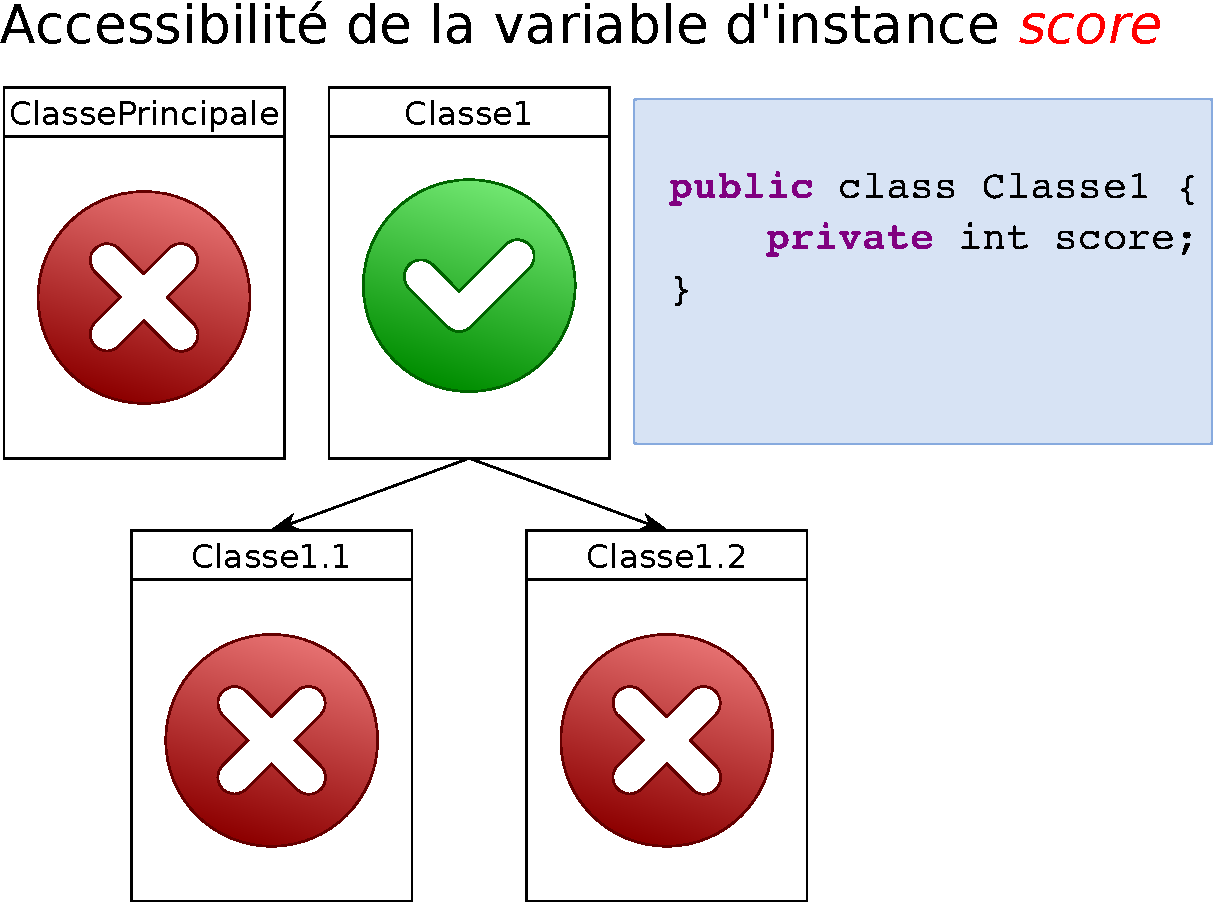
\includegraphics[width=0.3\textwidth]{figures/portee_private.pdf}}
\caption{Illustration de la portée des variables dans une classe}\label{fig:portee}
\end{figure}

\subsection{Variable de classe}
Tout d'abord les \gras[variable!de classe]{variables de classes}, qui sont définies dans la classe, avec l'attribut \gras{static}. Cette variable sera commune à toutes les instances de la classe. On déclare une variable de classe de la façon suivante :
\begin{lstlisting}[language=java]
public class Ville {
 
  /**
   * Variable de classe
   */
  static String nomVille;
\end{lstlisting}\index{static}

\bigskip

Pour accéder à une \gras[variable!de classe]{variable de classe} \textbf{var} (de la classe \textbf{Ville} par exemple) à l'intérieur même de celle-ci (ou une de ses instances), on y accède via :
\begin{lstlisting}[language=java]
Ville.var
\end{lstlisting}

\subsection{Méthode de classe}\label{sec:methode_classe}
Toutes les \textbf{méthodes} d'une \textbf{classe} n'utilisant que des \gras[variable!de classe]{variables de classes} doivent être déclarées \gras{static} ! On les appelle des \textbf{méthodes de classes} car elles sont globales à toutes vos instances !

\begin{remarque}
Par contre ceci n'est plus vrai si une méthode utilise des variables d'instances et des variables de classes...
\end{remarque}

L'\gras{accesseur} d'une \gras[variable!de classe]{variable de classe} doit aussi être déclarée \gras{static}, c'est une règle !

\subsection{Héritage}\index{héritage}\label{sec:heritage}
L'\gras{héritage} permet de créer des classes filles d'une classe donnée. L'intérêt de l'héritage est que toutes les méthodes et variables créées pour la classe parente se retrouveront dans les classes filles. 

\begin{lstlisting}[language=java]
class Capitale extends Ville {
 
private String president;
 
 /**
  *Constructeur par defaut
  */
  public Capitale(){
    //Ce mot cle appelle le constructeur de la classe mere.  
    super();
    president = "aucun";
  }
}
\end{lstlisting}\index{extends}

Pour plus de détails sur \gras{super()} voir \refsec{sec:surcharge}. \refsec{sec:empecher_heritage} détaille comment empêcher l'héritage.

\subsection{Généricité}\index{généricité}
La généricité, c'est pouvoir créer une classe qui puisse travaille avec n'importe quel type d'objet sans avoir à créer une classe différente à chaque fois. La particularité, c'est qu'une fois instancié, le type de variable utilisable par l'objet ne peut pas changer (chaque instance de la classe peut avoir un type de variable différent, mais une fois définit, on ne peut pas le changer). 

L'astuce est ici de définir une variable \texttt{T} pour désigner le type avec lequel travaille la classe. Exemple :
\begin{lstlisting}[language=java]
public class Solo<T> {
 
  /**
    * Variable d'instance
    */
  private T valeur;
  
  /**
    * Constructeur par defaut
    */
  public Solo(){
    this.valeur = null;
  }
  
  /**
    * Constructeur avec parametre
    * Inconnu pour l'instant
    * @param val
    */
  public Solo(T val){
    this.valeur = val;
  }
  
  
  /**
    * Definit la valeur avec le parametre
    * @param val
    */
  public void setValeur(T val){
    this.valeur = val;
  }
  
  /**
    * retourne la valeur deja "castee" par la signature de la methode !
    * @return
    */
  public T getValeur(){
    return this.valeur;
  }       
}
\end{lstlisting}

Dans cette classe, le \texttt{T} n'est pas encore défini. Vous le ferez à l'instanciation de cette classe. Par contre, une fois instancié avec un type, l'objet ne pourra travailler qu'avec le type de données que vous lui avez spécifié !
\begin{exemple}
\begin{lstlisting}[language=java]
public class Test {
 
  public static void main(String[] args) {
    // TODO Auto-generated method stub
    Solo<Integer> val = new Solo<Integer>(12);
    int nbre = val.getValeur();
    Solo<String> valS = new Solo<String>("TOTOTOTO");
    Solo<Float> valF = new Solo<Float>(12.2f);
    Solo<Double> valD = new Solo<Double>(12.202568);  
}
}
\end{lstlisting}
\end{exemple}

\bigskip

On n'est pas limité à une seule variable. On peut définir par ce même principe, plusieurs variables génériques dans une classe donnée : 
\begin{lstlisting}[language=java]
public class Duo<T, S> {
 
  /**
    * Variable d'instance de type T
    */
  private T valeur1;
  /**
    * Variable d'instance de type S
    */
  private S valeur2;
}
\end{lstlisting}
que l'on utilise de la façon suivante :
\begin{lstlisting}[language=java]
Duo<String, Boolean> dual = new Duo<String, Boolean>("toto", true);
System.out.println("Valeur de l'objet dual: val1 = " + dual.getValeur1() + ", val2 = " + dual.getValeur2());

Duo<Double, Character> dual2 = new Duo<Double, Character>(12.25895, 'C');
System.out.println("Valeur de l'objet dual2: val1 = " + dual2.getValeur1() + ", val2 = " + dual2.getValeur2()); 
\end{lstlisting}

\bigskip

On peut contourner l'interdiction d'utiliser un type différent en utilisant le point d'interrogation \og ?\fg lors de la déclaration du type des variables. Ça permet, pour une même variable, d'accepter l'écrasement de l'objet existant par un nouvel objet de type différent (mais l'objet défini n'acceptera toujours qu'un seul type de variable. 

\begin{exemple}
\begin{lstlisting}[language=java]
Duo<?, ?> dual = new Duo<String, Boolean>("toto", true);

System.out.println("Valeur de l'objet dual: val1 = " + dual.getValeur1() + ", val2 = " + dual.getValeur2());
dual = new Duo<Double, Character>();
dual = new Duo<Integer, Float>();
dual = new Duo<Solo, Solo>();
\end{lstlisting}
\end{exemple}


\section{Les instances de classe}
\subsection{Variable d'instance}
Il y a ensuite les \gras[variable!d'instance]{variables d'instance}, qui sont définies dans la classe. Cette variable \textbf{var} est accessible, à l'intérieur de la classe via \textbf{this.var} où \gras{this} désigne l'instance de classe. On défini une variable d'instance dans l'entête de la classe, de la façon suivante :
\begin{lstlisting}[language=java]
public class Ville {
 
  /**
   * Variable d'instance
   */
  String nomVille;
\end{lstlisting}

Pour accéder à une variable d'instance à l'intérieur d'une instance, on procède de la façon suivante :
\begin{lstlisting}[language=java]
this.var
\end{lstlisting}

Pour y accéder depuis l'extérieur, il est conseillé de configurer des accesseurs \og getVariable()\fg, voir \refsec{sec:good_behavior} pour plus de détails. On peut créer des variables privées (notamment pour faire des variables locales) en rajoutant un attribu privé à une variable. Il est recommandé de définir ces variables avec l'attribut \gras{private} et de créer des \gras[accesseur]{accesseurs} et des \gras[mutateur]{mutateurs} afin de voir le contenu de la variable et de le modifier.

\subsection{Méthodes d'instance}\label{sec:methode_instance}

\begin{figure}[htb]
\centering
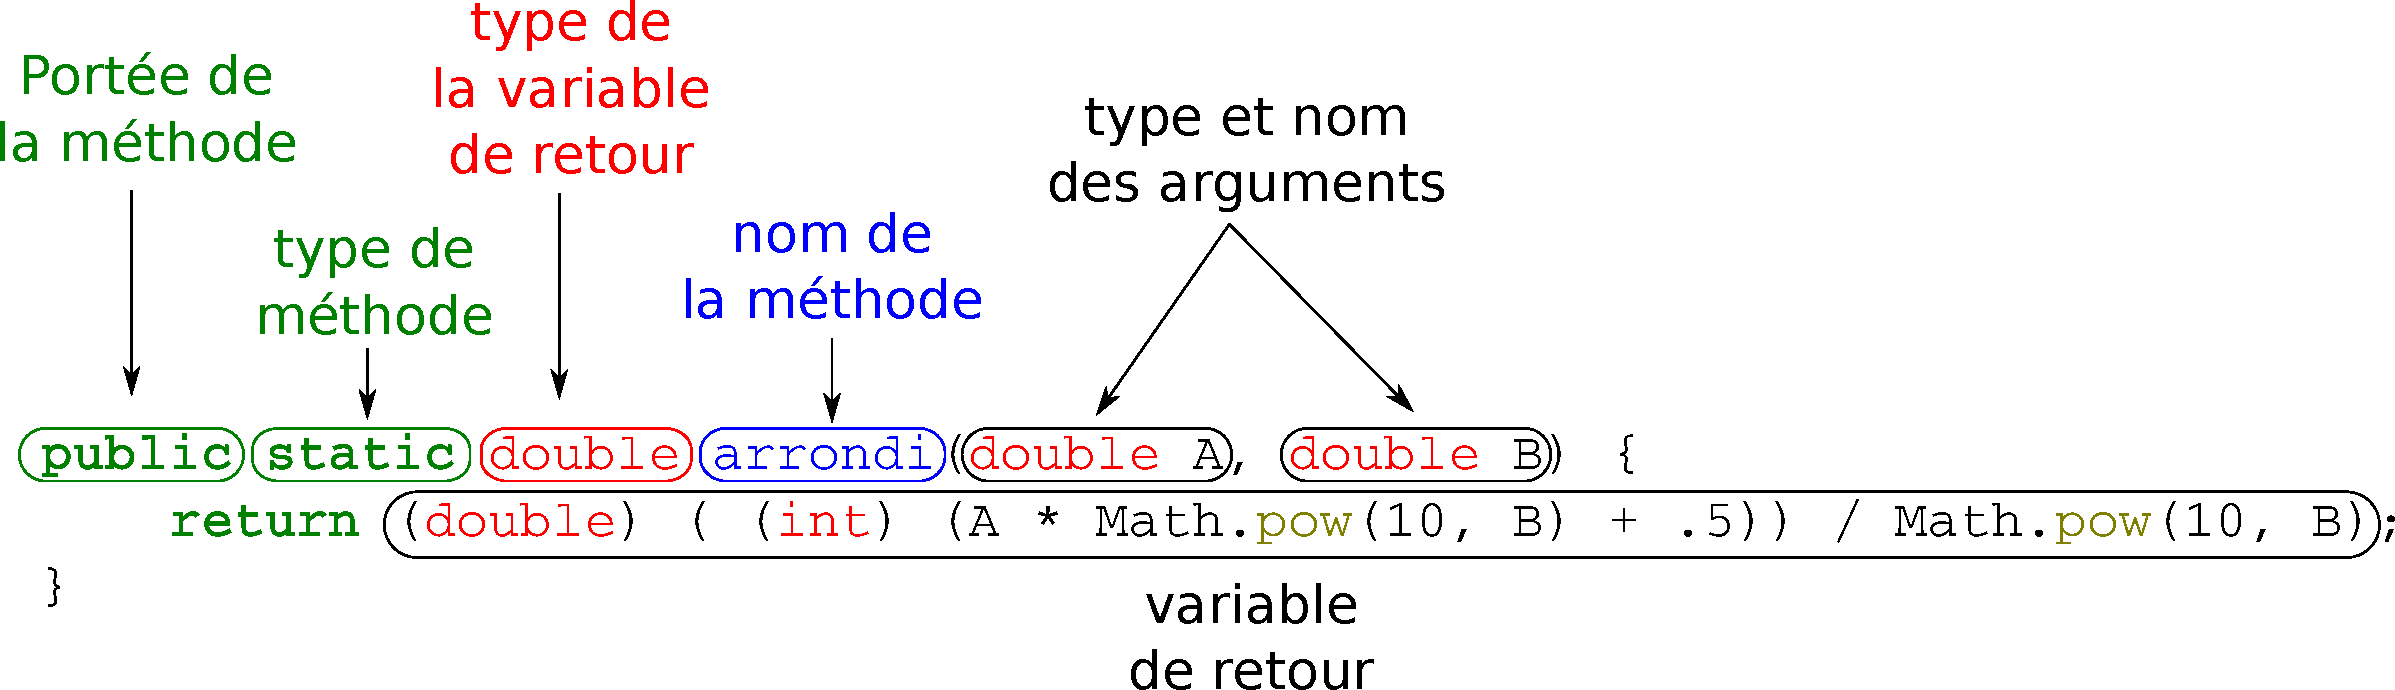
\includegraphics[width=\linewidth]{figures/method_scheme.pdf}
\caption{Explication des différents attributs d'une méthode. Le but ici est de présenter à quoi correspond la syntaxe, sans présenter les différents choix possibles.}
\end{figure}

Les méthodes ne sont pas limitées en nombre de paramètres (s'il n'y a pas d'argument, il faut au minimum \og \texttt{String[] args}\fg.

Il existe trois grands types de méthodes : 
\begin{itemize}
\item celles qui ne renvoient rien. Elles sont de type \gras{void}. Ces types de méthodes n'ont pas d'instruction \textbf{return} !
\item celles qui retournent des types primitifs (\gras[type!double]{double}, \gras[type!int]{int}...). Elles sont de type \gras[type!double]{double}, \gras[type!int]{int}, \gras[type!char]{char}... Celles-ci ont une instruction \textbf{return}.
\item celles qui retournent des objets. Par exemple, une méthode qui retourne un objet de type \gras[type!String]{String}. Celles-ci aussi ont une instruction \textbf{return}.
\end{itemize}

\bigskip

\begin{remarque}
On n'imbrique pas les méthodes et elles doivent toutes faire partie d'une classe. 
\end{remarque}

\begin{attention}
Les méthodes de la classe \textbf{main}, c'est à dire la classe lancée par défaut au début du programme et qui contient le \gras{main()}, doivent être \gras{static}
\end{attention}

\subsection{Accéder aux méthodes et variables d'un objet}
En règle générale, on appelle des méthodes ou des paramètres grâce à notre variable qui nous sert de référence, celle-ci suivie de l'opérateur ".", puis du nom de la dite méthode/variable.
\begin{lstlisting}[{language=java}]
String str = new String("opizrgpinbzegip");
str = str.subString(0,4);
\end{lstlisting}

Mais pour accéder aux données ou méthode de notre objet à l'intérieur même de celui-ci, cette méthode n'est pas possible. Pour y remédier, il faut utiliser le mot-clé \gras{this} :
\begin{lstlisting}[language=java]
public class Ville {
  
  /**
  * Variable d'instance
  */
  String nomVille;
  
  public Ville(String nom) {
    this.nomVille = "nom";
  }
}
\end{lstlisting}
où \textbf{this} désigne l'instance courante de l'objet (qui n'existe pas au moment de l'écriture du programme, mais qui existera quand le mot clé \textbf{this} aura besoin de pointer vers quelque chose. 


\section{Les méthodes}
Pour des infos sur les méthodes de classes (\refsec{sec:methode_classe}) et les méthodes d'instance (\refsec{sec:methode_instance}), se référer aux sections correspondantes.
\subsection{La surcharge de méthode}\label{sec:surcharge}
La surcharge de méthode consiste à garder un nom de méthode (donc un type de traitement à faire, pour nous, lister un tableau) et de changer la liste ou le type de ses paramètres.

Nous allons surcharger notre méthode afin qu'elle puisse travailler avec des \textbf{int} par exemple :
\begin{lstlisting}[language=java]
static void parcourirTableau(String[] tab)
  {
     for(String str : tab)
        System.out.println(str);
  }
        
static void parcourirTableau(int[] tab)
  {
     for(int str : tab)
        System.out.println(str);
  }
\end{lstlisting}

On peut aussi faire de même avec les tableaux à 2 dimensions ou ajouter des paramètres à la méthode.

\bigskip

Le mot-clé \gras{super()} permet de faire appel à la version parente d'une méthode donnée que l'on souhaite surcharger. Ça signifie concrêtement que \gras{super()} va exécuter la version parente de la méthode en lieu et place du mot-clé. Ceci fonctionne bien entendu pour le constructeur, ce qui permet d'initialiser la classe parente de manière normale, tout en rajoutant l'initialisation des variables propre à la classe courante : 
\begin{lstlisting}[language=java]
class Capitale extends Ville {
 
private String president;
 
 /**
  *Constructeur par defaut
  */
  public Capitale(){
    //Ce mot cle appelle le constructeur de la classe mere.  
    super();
    president = "aucun";
  }
}
\end{lstlisting}

\begin{remarque}
Dans le cas d'une méthode qui nécessite une variable, imaginez que \gras{super()} se comporte comme un alias. Il suffit de mettre en paramètre de \gras{super()} les valeurs que vous souhaitez : 
\begin{lstlisting}[language=java]
super(nom, hab, pays);
\end{lstlisting}
\end{remarque}

Pour aller plus loin, voir \refsec{sec:empecher_heritage} pour apprendre comment empêcher la surcharge et l'héritage

\subsection{Polymorphisme}\index{polymorphisme}
Le \gras{polymorphisme}, c'est le fait qu'une même méthode soit implémentée dans plusieurs classes, autorisant cette méthode à être utilisée indifféremment sur plusieurs types d'objets. 

\begin{attention}
Il ne faut pas confondre le \gras{polymorphisme}, c'est à dire le fait de définir une même méthode avec un squelette identique (même nombre et type d'arguments) dans plusieurs classes avec la surcharge de méthodes, qui permet au sein d'une même classe de définir la même méthode plusieurs fois mais avec un nombre ou type d'argument différents.
\end{attention}

Le polymorphisme permet d'agir sur la classe mère, dans laquelle les méthodes sont définies, et agir indifféremment sur des objets de sous-classes ayant redéfini les méthodes de la classe mère. 

\begin{remarque}
L'utilisation d'\gras[interface]{interfaces} permet aussi d'utiliser le polymorphisme dans des classes non issues de la même classe mère (voir \refsec{sec:interface}).
\end{remarque}

\subsection{Méthode abstraite}\label{sec:methode_abstraite}
Le mot-clé \gras{abstract} permet de créer une classe ou une méthode abstraite. Une méthode abstraite n'a pas de corps.

\begin{lstlisting}[language=java]
abstract class Animal{
   abstract void manger();//une methode abstraite
}
\end{lstlisting}

\begin{remarque}
Une classe déclarée abstraite n'est plus instanciable, mais elle n'est nullement obligée d'avoir des méthodes abstraites ! En revanche, une classe ayant une méthode abstraite doit être déclarée abstraite ! 
\end{remarque}

\section{Les classes : avancé}
\subsection{Empêcher la surcharge de méthode ou l'héritage}\label{sec:empecher_heritage}
En déclarant le mot-clé \gras{final} comme attribut d'une méthode, on empêche la surchage de méthode. Ces méthodes sont figées et vous ne pourrez \textit{jamais} redéfinir une méthode déclarée \gras{final}. Un exemple de ce type de méthode est la méthode \textbf{getClass()} de la classe \textbf{Object}.

\begin{remarque}
Il existe aussi des classes déclarées \gras{final}. Vous avez compris que ces classes sont immuables... Et vous ne pouvez donc pas faire hériter un objet d'une classe déclarée \gras{final}.
\end{remarque}

\subsection{Super-classes non instantiables : Classe abstraite}\label{sec:classe_abstraite}
Le mot-clé \gras{abstract} permet de créer une classe ou une méthode abstraite. Ça signifie concrêtement que la classe ne peut pas être instanciée. Elle n'est utile que pour définir des sous classes, ayant des méthodes ou attributs communs qu'on peut définir dans cette super-classe qui n'est pas utilisable en l'état.
\begin{exemple}
Imaginez une méta-classe abstraite \textbf{Animal} qui servirait à définir des sous classes \textbf{Chien}, \textbf{Chat}, \textbf{Lion}, \textbf{Ours} etc...
\end{exemple}

\begin{lstlisting}[language=java]
abstract class Animal{
 
}
\end{lstlisting}

Une telle classe peut avoir le même contenu qu'une classe normale. Ses enfants pourront utiliser tous ses éléments déclarés (attributs et méthodes) public. Cependant, ce type de classe permet de définir des méthodes abstraites, voir \refsec{sec:methode_abstraite}.

\begin{remarque}
Les classes abstraites sont à utiliser lorsque qu'une classe mère ne doit pas être instanciée.
\end{remarque}

\subsection{Compilations de définitions de méthodes : Interfaces}\label{sec:interface}\index{interface}
Une \gras{interface} permet de définir le squelette (le nom de la méthode, le nombre et le type des arguments) de différentes méthodes généralistes. Ensuite, un peu comme un module, on appelle cette interface dans la classe voulue. On doit alors implémenter \textit{toutes} les méthodes définies dans l'interface.

On définit une interface \textbf{I} de la façon suivante :
\begin{lstlisting}[language=java]
public interface I{
 
   public void A();
   public String B();
 
}
\end{lstlisting}

On appelle une \gras{interface} \textbf{I} dans la classe \textbf{X}
\begin{lstlisting}[language=java]
public class X implements I{
    public void A(){
      //.......
    }
 
    public String B(){
      //.......
    }
}
\end{lstlisting}

\subsection{Conversion d'objets}
Il est possible, en particulier pour l'utilisation de certaines méthodes, de convertir des objets. Imaginons qu'on ait une classe \textbf{Ville}, définissant la méthode \textbf{.decrisToi()}, le code suivant est possible :
\begin{lstlisting}[language=java]
//Def d'un tableau de ville null
Ville[] tableau = new Ville[6];

/*
On initialise les objets dans cette partie non ecrite
*/

//il ne nous reste plus qu'a decrire tout notre tableau !
for(Object v : tableau){
  System.out.println(((Ville)v).decrisToi()+"\n");
}
\end{lstlisting}
On a ainsi converti la variable \textbf{v} afin de pouvoir utiliser la méthode \textbf{decrisToi()} qui n'existe pas dans la classe \textbf{Object}. Ceci fonctionne sans doute parce que la classe Object est la classe parente de toute classe par défaut, c'est à dire que toute classe :
\begin{lstlisting}[language=java]
class Ville {

}
\end{lstlisting}
est en fait équivalente à :
\begin{lstlisting}[language=java]
class Ville extends Object {

}
\end{lstlisting}

Pour plus de détails sur \gras{extends}, voir \refsec{sec:heritage}.

\subsection{Covariance des variables}
Il existe ce qu'on appelle la \gras{covariance des variables}, c'est à dire qu'il est possible d'utiliser une variable, déclarée comme appartenant à une classe \textbf{ClasseParente}, pour stocker une instance de n'importe quel objet d'une classe héritée \textbf{ClasseFille}. Un exemple :
\begin{lstlisting}[language=java]
//Def d'un tableau de ville null
Ville[] tableau = new Ville[6];
    
//Definition d'un tableau de noms de Villes et d'un tableau de nombres d'habitants
String[] tab = {"Marseille", "lille", "caen", "lyon", "paris", "nantes"};
int[] tab2 = {123456, 78456, 654987, 75832165, 1594,213};

/* Les 3 premiers elements du tableau seront des Villes, et le reste, des capitales
*/
for(int i = 0; i < 6; i++){
  if (i <3){
    Ville V = new Ville(tab[i], tab2[i], "france" );
    tableau[i] = V;
  }

  else{
    Capitale C = new Capitale(tab[i], tab2[i], "france", "Sarko");
    tableau[i] = C;
  }
}

//il ne nous reste plus qu'a decrire tout notre tableau !
for(Ville v : tableau){
  System.out.println(v.decrisToi()+"\n");
}
\end{lstlisting}

\section{Eclipse}
Il est impossible de faire un tutoriel Java sans s'attarder sur Eclipse, excellent logiciel pour coder en Java et qui facilite vraiment la vie des développeurs.

\subsection{Générer automatiquement les accesseurs et les mutateurs avec Eclipse}\index{accesseur}\index{mutateur}\index{Eclipse}
Une fois qu'on a créé une classe avec beaucoup de variables d'instances ou de classe, \gras{eclipse} permet de générer automatiquement les \gras[accesseur]{accesseurs} et les \gras[mutateur]{mutateurs}. 

Il faut pour cela aller dans le menu \textbf{Source}, puis l'option générale \textbf{Generate Getters and Setters}. \gras{Eclipse} propose alors la liste des variables présentes dans la classe courante.

\subsection{Récupérer un projet déjà existant sur un SVN distant}\index{SVN}
Il faut installer le plugin \gras{subclipse} au préalable.

Il faut pour celà créer un nouveau ``Projet'' : File>New>Other>Checkout projet from SVN (dans le dossier SVN).

Suivre les instructions et renseigner l'adresse du dépot SVN (sans mettre le nom du sous-dossier où se trouve le projet). Dans l'onglet suivant, vous pourrez spécifiez le nom du dossier qui vous intéresse.

\subsection{Synchroniser un projet en le sauvegardant sur un SVN distant}
En prenant un projet déjà existant localement (mais qui n'existe pas sur le SVN distant). Il faut faire clic droit sur le nom du projet. Puis \textbf{Team} et enfin \textbf{Share Project...}

\printindex
\end{document}